\documentclass[aspectratio=169,11pt]{beamer}
\usepackage[UTF8,fontset=none]{ctex}
\setCJKmainfont{Microsoft JhengHei}
\setCJKsansfont{Microsoft JhengHei}
\usepackage{amsmath,amssymb,booktabs,array}
\usepackage{pgfplots}
\pgfplotsset{compat=1.18}
\definecolor{navy}{HTML}{183750}
\definecolor{teal}{HTML}{007E87}
\definecolor{orange}{HTML}{B45A20}
\setbeamercolor{normal text}{fg=navy,bg=white}
\setbeamercolor{structure}{fg=teal}
\setbeamercolor{frametitle}{fg=navy}
\setbeamercolor{alerted text}{fg=orange}
\setbeamerfont{frametitle}{size=\Large,series=\bfseries}
\setbeamertemplate{navigation symbols}{}
\setbeamertemplate{itemize items}[circle]
\setbeamersize{text margin left=8mm,text margin right=8mm}
\setbeamertemplate{footline}{\hspace{8mm}\scriptsize Handout 4 自讀筆記\hfill\insertsectionhead\hfill\insertframenumber/\inserttotalframenumber\hspace{8mm}\vspace{3mm}}
\newcommand{\src}[1]{\par\vfill{\scriptsize\color{teal}#1}}
\newcommand{\slide}[3]{\begin{frame}[t]{#1}#3\src{#2}\end{frame}}
\newcommand{\bi}{\begin{itemize}\setlength{\itemsep}{5pt}}
\newcommand{\ei}{\end{itemize}}
\newcommand{\key}[1]{\par\medskip{\color{teal}\bfseries #1}\par\smallskip}
\newcommand{\dd}{\mathrm{d}}
\newcommand{\bookslide}[3]{\slide{#1}{課本：#2。頁碼為書本印刷頁碼}{#3}}
% Original images extracted losslessly from the supplied textbook PDF.
\newcommand{\originalfigure}[6]{
\begin{frame}[t]{課本原圖 #1：#2}
\centering
\includegraphics[width=.94\linewidth,height=5.05cm,keepaspectratio]{figures/#4}\par
\vspace{2mm}\raggedright\small #5\par
\vfill{\scriptsize\color{teal}原圖：Collinson, 第 3 版，Fig. #1，p. #3。#6}\par
\end{frame}}


\newcommand{\handoutfigure}[3]{
\begin{frame}[t]{講義原頁 #1：#2}
\centering
\includegraphics[width=.97\linewidth,height=5.65cm,keepaspectratio]{figures/#3}\par
\vfill{\scriptsize\color{teal}原圖與文字：賴盈誌老師提供之 Handout，PDF 第 #1 頁。}\par
\end{frame}}
\title{飛機動力學、線性模型與增穩}
\subtitle{Handout 4\\繁體中文自讀詳解}
\author{依賴盈誌老師課程講義整理}
\date{CA7528 Digital Avionics\quad Fall 2026}
\begin{document}
\begin{frame}\titlepage\centering\small 概念、原圖、推導、算例與自我檢查\end{frame}
\section{閱讀地圖}
\slide{範圍與閱讀方式}{Handout 4，PDF pp. 1--68}{
\bi
\item Handout 4 與既有 Chapter 3 的運動方程、響應、PCU 及 SAS 推導。
\item 原頁碼一律指講義 PDF 頁序。標示「課本」的頁碼則是 Collinson 第三章印刷頁碼。
\item 先讀概念，再對照原圖。自我檢查先遮住參考解答，再獨立計算或口頭說明。
\item 自編算例與補充推導依題內假設使用。歷史機型、服務與表格依原教材背景理解。
\ei
}
\slide{分次閱讀安排}{Handout 4 閱讀地圖}{
\small
\bi
\item \textbf{講義導讀}：模型與飛行品質的關係。
\item \textbf{講義核對}：角速度與 Euler 角變化率、剛體假設與慣性乘積、控制面也會產生力、狀態空間中的輸出與可量測性、SAS 的阻尼方向。
\item \textbf{算例與響應}：二階分母與傳遞函數。
\ei
}
\slide{公式推導與詳解閱讀地圖}{Collinson 第三章對應主題；課本頁碼於各頁標示}{
\small
\bi
\item 3.4 運動方程與氣動導數：旋轉座標、線性化、導數單位及縱向／橫向狀態模型。
\item 3.5 縱向響應：短週期近似、傳遞函數、阻尼、零點及算例重算。
\item 3.6 橫向控制：轉彎、滾轉、偏航及動態模態。
\item 3.7 動力操縱與 PCU：液壓伺服、位置回授及頻寬。
\item 3.8 SAS：角速度回授、wash-out、增益排程及備援。
\item 講義核對與自我檢查：假設、控制力、輸出量測與阻尼方向。
\ei
}
\section{講義導讀}
\slide{模型與飛行品質的關係}{Handout 4，PDF pp. 1--12；概念整理與補充推導}{
\small
\bi
\item 飛機模型把操縱命令、飛機狀態與輸出關係寫成可分析的方程，操縱品質則加入任務與飛行員需求。
\item 機體座標便於表示感測、氣動及控制輸入，地面或導航座標便於表示位置與航跡。
\item 直線平飛分析可使用局部平地近似，但不能直接套用到長距離導航。
\ei
\key{閱讀重點}先建立六自由度模型，再以小擾動近似分析響應，最後考慮致動器與增穩回授。
}
\handoutfigure{6}{模型與飛行品質的關係}{handout04-p006.png}
\handoutfigure{9}{模型與飛行品質的關係}{handout04-p009.png}
\slide{自我檢查：模型與飛行品質的關係}{依 Handout 範圍自編問題與參考解答}{
\small
\key{先自行作答}
六自由度的六個方程，為什麼不代表完整狀態模型只有六個狀態？
\key{參考解答}
六自由度描述三平移與三旋轉。要從速度及角速度求姿態與位置，還需運動學方程，加入致動器或引擎動態後狀態數還會增加。
}
\section{3.4 運動方程與氣動導數}
\bookslide{六自由度與機體座標}{3.4.1，pp. 115--116}{
\small
原點設在 CG，$x$ 朝前、$y$ 朝右翼、$z$ 朝下，採右手座標系。
\begin{center}\begin{tabular}{ccccc}
\toprule 軸 & 平移速度 & 角速度 & 力 & 力矩\\\midrule
$x$ & $U$ & $p$：roll & $X$ & $L$\\
$y$ & $V$ & $q$：pitch & $Y$ & $M$\\
$z$ & $W$ & $r$：yaw & $Z$ & $N$\\\bottomrule
\end{tabular}\end{center}
\bi\item 正 $p$ 為右翼下降，正 $q$ 為抬頭，正 $r$ 為機頭向右。
\item 機體座標適合短期控制模型，也與機載陀螺儀、加速度計的量測軸一致。
\item 地理／慣性座標適合描述航跡與導航。兩者需透過姿態轉換連接。\ei
}
\originalfigure{3.15}{機體軸、速度與操縱面}{116}{fig-3-15.png}{對照軸向、角速度與控制面符號，尤其注意 z 軸朝下。}{}

\bookslide{旋轉座標系中的加速度}{3.4.1，pp. 116--117，式 (3.13)--(3.15)}{
\[\mathbf a_B=\dot{\mathbf V}_B+\boldsymbol\omega_B\times\mathbf V_B,
\qquad\mathbf V_B=\begin{bmatrix}U\\V\\W\end{bmatrix},\quad
\boldsymbol\omega_B=\begin{bmatrix}p\\q\\r\end{bmatrix}.\]
\[\begin{aligned}
a_x&=\dot U-Vr+Wq,\\
a_y&=\dot V+Ur-Wp,\\
a_z&=\dot W-Uq+Vp.
\end{aligned}\]
\key{物理意義}機體座標本身會旋轉。即使速度分量瞬間不變，速度向量在慣性空間仍可能改變方向，所以不能只用 $\dot U,\dot V,\dot W$ 表示加速度。
}
\originalfigure{3.16}{座標旋轉造成的速度變化}{117}{fig-3-16.png}{將圖上的微小向量變化連到角速度與速度向量的叉積項。}{}

\bookslide{Euler 角與旋轉次序}{3.4.2，pp. 118--119}{
\bi
\item 姿態以偏航 $\psi$、俯仰 $\theta$、滾轉 $\phi$ 描述，依序施加 yaw、pitch、roll 旋轉。
\item 三維旋轉通常不可交換次序。相同三個角度，改變次序會得到不同姿態。
\item 陀螺儀量到的是機體角速度 $p,q,r$，一般不等於 Euler 角變化率。
\ei
\[\begin{aligned}
p&=\dot\phi-\dot\psi\sin\theta,\\
q&=\dot\theta\cos\phi+\dot\psi\cos\theta\sin\phi,\\
r&=\dot\psi\cos\theta\cos\phi-\dot\theta\sin\phi.
\end{aligned}\]
}
\originalfigure{3.17}{Euler 姿態角}{118}{fig-3-17.png}{區分姿態角與機體角速度，並留意旋轉次序的重要性。}{}

\bookslide{Euler 角速度的反解}{3.4.2，p. 119；補充代數反解}{
\[\begin{bmatrix}\dot\phi\\\dot\theta\\\dot\psi\end{bmatrix}
=\begin{bmatrix}
1&\sin\phi\tan\theta&\cos\phi\tan\theta\\
0&\cos\phi&-\sin\phi\\
0&\sin\phi/\cos\theta&\cos\phi/\cos\theta
\end{bmatrix}\begin{bmatrix}p\\q\\r\end{bmatrix}.\]
\bi
\item 近水平、小角度擾動下，$\dot\phi\simeq p$、$\dot\theta\simeq q$、$\dot\psi\simeq r$。
\item 大坡度轉彎時，$q$ 會含偏航角變化的投影，不能直接令 $q=\dot\theta$。
\item $\cos\theta=0$ 使此組參數化奇異。這是 Euler 角描述的限制，並非飛機物理運動無法存在。
\ei
}
\bookslide{小擾動線性化的起點}{3.4.3，pp. 119--122}{
\[U=U_0+u,\qquad V=v,\qquad W=W_0+w.\]
\bi
\item 參考狀態為等速、平直、配平飛行，無側滑與角速度。$u,v,w,p,q,r$ 為偏離此狀態的小量。
\item 捨棄二階小量乘積，例如 $vr,uq,wp$。保留 $U_0r,W_0q$，因為 $U_0,W_0$ 是參考值。
\item $W_0$ 不必為零：機體 $x$ 軸若未與速度向量重合，配平速度仍有 $z$ 軸分量。
\item 模型只在指定配平點附近成立。高度、速度、Mach 數或構型改變時，係數也會改變。
\ei
}
\originalfigure{3.18}{飛機受到的外力}{120}{fig-3-18.png}{配平時各方向的合力為零，擾動模型處理的是力的增量。}{}

\bookslide{小擾動力與力矩方程}{3.4.3，pp. 121--122，式 (3.22)--(3.27)}{
\small
扣除配平狀態的合力與合力矩，且配平俯仰角很小時：
\[\begin{aligned}
X_a-mg\theta&=m(\dot u+W_0q),\\
Y_a+mg\phi&=m(\dot v-W_0p+U_0r),\\
Z_a&=m(\dot w-U_0q).
\end{aligned}\]
\[L=I_x\dot p,\qquad M=I_y\dot q,\qquad N=I_z\dot r.\]
\bi
\item $-mg\theta$ 與 $mg\phi$ 來自重力在旋轉後機體軸上的分量變化。
\item 角運動式採教材的主慣性軸近似，使慣性積為零，並忽略角速度乘積。
\item 只有左右對稱，不足以保證任選機體軸的 $I_{xz}$ 必定為零。\ei
}
\originalfigure{3.19}{氣動力、推力與重力分量}{121}{fig-3-19.png}{對照重力投影與三軸力矩，核對運動方程中的符號。}{}

\bookslide{氣動導數就是局部偏導數}{3.4.4，pp. 122--123}{
\[\Delta F\simeq\sum_i\left.\frac{\partial F}{\partial x_i}\right|_{\rm trim}\Delta x_i.\]
例如 $X_u=\partial X/\partial u$，表示其他變數固定時，前向速度小幅改變造成的 $x$ 方向力變化率。
\[X_a\simeq X_u u+X_w w,\qquad M\simeq M_w w+M_q q+M_\eta\eta+\cdots\]
\bi
\item 下標指出「對哪個變數微分」，前面的字母指出「哪種力或力矩」。
\item 導數必須在指定飛行狀態、構型與 CG 位置附近使用。
\item 各導數可由分析、試驗或辨識取得。局部線性不代表整個飛行包線都線性。
\ei
}
\bookslide{導數的單位與角度轉換}{3.4.4，pp. 123、130--131；補充單位檢查}{
\small
\begin{tabular}{lll}
\toprule 導數 & 定義 & 單位\\\midrule
$X_u$ & $\partial X/\partial u$ & $\mathrm{N/(m/s)}$\\
$M_w$ & $\partial M/\partial w$ & $\mathrm{N\,m/(m/s)}$\\
$M_q$ & $\partial M/\partial q$ & $\mathrm{N\,m/(rad/s)}$\\
$M_\eta$ & $\partial M/\partial\eta$ & $\mathrm{N\,m/rad}$\\
$M_\alpha$ & $\partial M/\partial\alpha$ & $\mathrm{N\,m/rad}$\\\bottomrule
\end{tabular}
\[w\simeq U_0\alpha\quad\Longrightarrow\quad M_\alpha=U_0M_w,\quad Z_\alpha=U_0Z_w.\]
上述轉換假設參考 $x$ 軸近似對準速度方向，且 $U_0$ 固定。
\key{常見錯誤}有的資料先以 $m$ 或 $I_y$ 除過導數，有的使用無因次導數。拿到數值前先核對定義，避免重複除以慣性或漏掉尺度。
}
\bookslide{縱向導數：速度與迎角的作用}{3.4.4.1，pp. 124--125}{
\small
\begin{tabular}{p{.22\textwidth}p{.64\textwidth}}
\toprule 導數 & 物理來源\\\midrule
$X_u,\ Z_u$ & 速度改變動壓與氣動係數，使阻力、升力改變。\\
$X_w,\ Z_w$ & 垂直速度擾動改變迎角，進而改變升力與阻力。\\
$M_w$ & 迎角擾動引起俯仰力矩，是縱向靜穩定的重要指標。\\
$M_u$ & 速度改變引起俯仰力矩。教材視為相對小而省略。\\\bottomrule
\end{tabular}
\key{方向判斷}在 $z$ 向下、正迎角增加升力的慣例下，通常 $Z_w<0$。穩定配置通常有 $M_w<0$。導數仍應以實際座標、操作點與構型判定。
}
\bookslide{俯仰阻尼的來源}{3.4.4.1，p. 125，圖 3.20}{
尾翼距離 CG 為 $l_t$。機體有俯仰角速度 $q$ 時，尾翼產生切向速度，其大小約為 $l_tq$。
\[\Delta\alpha_t\simeq\frac{l_tq}{V_T}\]
\bi
\item 這個局部氣流角度改變尾翼升力，尾翼力再乘上 $l_t$ 形成俯仰力矩。
\item 阻尼力矩通常反抗當前角速度，所以帶符號的 $M_q<0$。
\item $Z_q q$ 是同一現象造成的垂直力，$M_q q$ 是其俯仰力矩。
\ei
\key{恢復與阻尼}迎角誤差引起 $M_\alpha\alpha$，角速度引起 $M_q q$。前者像彈簧，後者像阻尼器。
}
\originalfigure{3.20}{俯仰率造成的尾翼阻尼}{125}{fig-3-20.png}{尾翼切向速度改變局部迎角，其力矩反抗原來的俯仰運動。}{}

\bookslide{下洗延遲與控制導數}{3.4.4.1，pp. 125--126}{
\bi
\item 機翼迎角改變後，下洗變化需經過一段傳遞時間才作用於尾翼。
\item 教材以 $Z_{\dot w}\dot w$、$M_{\dot w}\dot w$ 近似這種非定常效果。
\item 升降舵或全動尾翼偏轉 $\eta$，產生 $Z_\eta\eta$ 的垂直力與 $M_\eta\eta$ 的俯仰力矩。
\item $\eta$ 的正方向取決於操縱面定義，不能只靠「正舵角」三個字推測力矩方向。
\ei
\[\begin{aligned}
X_a&=X_u u+X_w w,\\
Z_a&=Z_u u+Z_w w+Z_{\dot w}\dot w+Z_q q+Z_\eta\eta,\\
M&=M_w w+M_q q+M_{\dot w}\dot w+M_\eta\eta.
\end{aligned}\]
}
\bookslide{側滑力與風向標穩定}{3.4.4.2，pp. 126--128}{
\bi
\item 側滑速度 $v$ 使機身側面與垂直尾翼受到側向氣流，產生側向力 $Y_vv$。
\item 垂直尾翼的側力乘上距 CG 的力臂，產生使機頭對準相對氣流的恢復力矩。
\item 機身側向氣動作用可能抵銷尾翼的穩定作用，因此要看整機的 $N_v$。
\item 垂尾面積與力臂的乘積形成 fin volume，也須滿足非對稱推力等控制需求。
\ei
\key{本筆記的側滑符號}
後續狀態模型採 $\beta\simeq v/U_0$。在此慣例下，通常 $Y_v<0$、方向穩定時 $N_v>0$。教材 p. 152 的純偏航角度約定將另行說明。
}
\originalfigure{3.21}{側滑與側向力}{127}{fig-3-21.png}{區分機身側力和垂尾側力，以及它們關於 CG 的力矩。}{}

\bookslide{側滑如何產生滾轉}{3.4.4.2，p. 128，圖 3.22}{
\bi
\item 上反角（dihedral）使側滑時左右翼的有效迎角不同，升力差產生 $L_vv$。
\item 後掠翼也會讓側滑改變左右翼受流狀況，即使幾何上反角為零，仍可有側滑滾轉效應。
\item 垂尾側力的作用點若在滾轉軸上方，也會產生滾轉力矩。
\item 機身繞流與高／低翼布局會改變此效果。教材指出低翼布局通常需較大的幾何上反角。
\ei
\key{理解重點}上反角主要透過「側滑」影響滾轉。只有坡度角本身，不能直接替代側滑角來計算 $L_vv$。
}
\originalfigure{3.22}{上反角與側滑的作用}{128}{fig-3-22.png}{側滑改變左右翼有效迎角，升力差因而產生滾轉力矩。}{}

\bookslide{角速度導數與橫向耦合}{3.4.4.2，pp. 128--129}{
\small
\begin{tabular}{p{.16\textwidth}p{.71\textwidth}}
\toprule 項 & 形成機制\\\midrule
$L_pp$ & 滾轉造成左右翼垂直速度不同，形成反抗滾轉的升力差。通常 $L_p<0$。\\
$N_pp$ & 滾轉造成左右翼升力與阻力差，進而產生偏航力矩。\\
$N_rr$ & 偏航使垂尾產生局部側向速度，形成反抗偏航的力矩。通常 $N_r<0$。\\
$L_rr$ & 偏航使左右翼相對氣流速度不同，升力差造成滾轉力矩。\\\bottomrule
\end{tabular}
\key{為何要保留耦合}副翼引起的滾轉會影響偏航，偏航又影響側滑與滾轉，因此真實橫向響應不只有一個滾轉時間常數。
}
\originalfigure{3.23}{滾轉率造成的阻尼力矩}{129}{fig-3-23.png}{比較左右翼的局部速度與升力變化，辨認反抗滾轉的力矩。}{}

\bookslide{副翼與方向舵的控制導數}{3.4.4.2，pp. 129--130}{
\small
$\xi$ 為差動副翼偏轉，$\zeta$ 為方向舵偏轉。
\bi
\item $L_\xi$：副翼造成升力差，直接控制滾轉。
\item $N_\xi$：副翼伴隨阻力差，造成偏航耦合，可能需要方向舵協調。
\item $Y_\zeta,N_\zeta$：方向舵造成側向力與偏航力矩。
\item $L_\zeta$：方向舵側力等效作用高度等因素帶來滾轉力矩。
\ei
\[\begin{aligned}
Y_a&=Y_vv+Y_\zeta\zeta,\\
L&=L_vv+L_pp+L_rr+L_\xi\xi+L_\zeta\zeta,\\
N&=N_vv+N_pp+N_rr+N_\xi\xi+N_\zeta\zeta.
\end{aligned}\]
}
\bookslide{縱向與橫向何時可以分開？}{3.4.4--3.4.5，pp. 123--131}{
\bi
\item 對稱飛機、對稱的平直配平狀態，以及小擾動線性化，使縱向與橫向可以近似解耦。
\item 縱向組：前向速度 $u$、垂直速度 $w$、俯仰角速度 $q$ 與姿態 $\theta$。
\item 橫向組：側滑速度 $v$、滾轉角速度 $p$、偏航角速度 $r$ 與坡度 $\phi$。
\item 大迎角、大幅度動作、非對稱掛載、強耦合或非對稱配平時，此分法可能不足。
\ei
\key{階數提醒}「三條動力學方程」不代表模型一定只有三個狀態。加入姿態運動學方程後，常見模型為四階。
}
\bookslide{完整線性縱向方程}{3.4.5，p. 131，式 (3.34)--(3.36)}{
\small
\[\begin{aligned}
m\dot u&=X_u u+X_w w-mW_0q-mg\theta,\\
(m-Z_{\dot w})\dot w&=Z_u u+Z_w w+(mU_0+Z_q)q+Z_\eta\eta,\\
I_y\dot q-M_{\dot w}\dot w&=M_w w+M_q q+M_\eta\eta,\\
\dot\theta&=q.
\end{aligned}\]
\bi
\item $\dot w$ 同時出現在垂直力與俯仰力矩方程，要先聯立整理，才能寫成標準狀態空間。
\item 可先寫成 $E\dot{\mathbf x}=A_0\mathbf x+B_0\eta$，若 $E$ 可逆，再求 $A=E^{-1}A_0$。
\item 教材後續示範會省略 $Z_q,Z_{\dot w},M_{\dot w}$，得到較清楚的四階矩陣。
\ei
}
\bookslide{縱向狀態空間模型}{3.4.5，pp. 131--133，式 (3.40)、(3.42)}{
\small
\[\mathbf x_\ell=\begin{bmatrix}u&w&q&\theta\end{bmatrix}^{T},
\qquad\dot{\mathbf x}_\ell=A_\ell\mathbf x_\ell+B_\ell\eta\]
\[A_\ell=\begin{bmatrix}
X_u/m&X_w/m&-W_0&-g\\
Z_u/m&Z_w/m&U_0&0\\
0&M_w/I_y&M_q/I_y&0\\
0&0&1&0
\end{bmatrix},\qquad
B_\ell=\begin{bmatrix}0\\Z_\eta/m\\M_\eta/I_y\\0\end{bmatrix}.\]
\bi
\item 最後一列為姿態運動學。$-g\theta$ 將姿態變化連接回前向速度。
\item $A$ 描述飛機自身動態，$B$ 描述控制輸入如何驅動狀態。
\item 矩陣中特定零元素來自本模型的省略，不是所有飛機都恆為零。
\ei
}
\bookslide{橫向狀態空間模型}{3.4.5，pp. 132--134，式 (3.41)、(3.43)}{
\small
\[\mathbf x_t=\begin{bmatrix}v&p&r&\phi\end{bmatrix}^{T},
\quad\mathbf u_c=\begin{bmatrix}\zeta&\xi\end{bmatrix}^{T}\]
\[\dot{\mathbf x}_t=
\begin{bmatrix}
Y_v/m&W_0&-U_0&g\\
L_v/I_x&L_p/I_x&L_r/I_x&0\\
N_v/I_z&N_p/I_z&N_r/I_z&0\\
0&1&0&0
\end{bmatrix}\mathbf x_t+
\begin{bmatrix}
Y_\zeta/m&0\\
L_\zeta/I_x&L_\xi/I_x\\
N_\zeta/I_z&N_\xi/I_z\\
0&0
\end{bmatrix}\mathbf u_c.\]
\key{物理對照}第一列含側力、旋轉座標項與重力側向分量。第二、三列相互耦合。最後一列是 $\dot\phi=p$。
}
\bookslide{由模型計算響應與模態}{3.4.5，pp. 132--134；補充特徵值觀點}{
\[\dot{\mathbf x}=A\mathbf x+B\mathbf u_c,\qquad
\mathbf x_{k+1}\simeq\mathbf x_k+\Delta t(A\mathbf x_k+B\mathbf u_{c,k}).\]
\bi
\item 教材用前向 Euler 法說明數值積分。$\Delta t$ 必須足夠小，並檢查縮小步長後結果是否收斂。
\item 自由響應的模態由 $A$ 的特徵值決定。負實部表示衰減，正實部表示發散。
\item 複數共軛根表示振盪。虛部決定振盪頻率，實部決定包絡衰減率。
\item 若輸出為 $y=C\mathbf x$，零初值下 $G(s)=C(sI-A)^{-1}B$。這把狀態空間接到傳遞函數。
\ei
}
\bookslide{本單元自我檢查}{3.4，pp. 115--134}{
\begin{enumerate}\setlength{\itemsep}{8pt}
\item 為何保留 $U_0r$ 卻捨棄 $ur$？\\
\textbf{前者是一階擾動項，後者是兩個小量相乘。}
\item $M_w$ 與 $M_q$ 分別代表什麼？\\
\textbf{迎角／垂直速度帶來的恢復力矩，以及俯仰角速度帶來的阻尼力矩。}
\item 有側滑時，是否只需要一條側向力方程？\\
\textbf{否，還會激發滾轉與偏航力矩。}
\item 不同飛行條件可否直接共用一組 $A,B$？\\
\textbf{只有局部近似合理時可以，否則須更新導數或採增益排程。}
\end{enumerate}
}

\section{3.5 縱向控制與響應}
\bookslide{升降舵輸入如何改變飛行路徑}{3.5.1，pp. 134--135}{
\bi
\item 升降舵／尾翼偏轉，先改變尾翼力與俯仰力矩。
\item 俯仰力矩使 $q$ 增加，機身旋轉使迎角改變，主翼升力隨之改變。
\item 新的升力提供使航跡彎曲的法向力。恢復力矩與俯仰阻尼限制響應。
\item 慣性使響應可能有過衝。固定輸入在短週期定速近似下，可對應近似固定的 $q$ 與迎角增量。
\ei
\key{精確一點}小角度下 $\alpha\simeq\theta-\gamma$，所以 $\dot\gamma=q-\dot\alpha$。只有迎角變化很慢時，航跡曲率加速度才近似 $a_n\simeq Uq$。
}
\originalfigure{3.24}{縱向機動的建立過程}{135}{fig-3-24.png}{從尾翼力矩、迎角變化，依序追到主翼升力與航跡彎曲。}{}

\bookslide{桿力每 g 與人工力感}{3.5.2，pp. 135--136}{
\bi
\item 動壓越高，相同迎角增量所產生的升力通常越大，因此每 $g$ 所需舵角與桿位移改變。
\item 教材指出高性能飛機的 stick displacement/$g$ 可能跨包線變化達約 40:1。
\item 純手動操縱時，飛行員可感到氣動鉸鏈力矩。全動力操縱隔離此力感，需要人工力感裝置。
\item 簡單彈簧提供桿力與位移關係；較完整的人工力感裝置依動壓調整剛度。
\ei
\key{設計目的}讓飛行員施力與希望得到的機動程度有可預期的關係，同時讓響應與阻尼在包線內維持可接受程度。
}
\bookslide{完整縱向響應的兩個時間尺度}{3.5.3，pp. 136--138}{
\[\frac{q(s)}{\eta(s)}
=\frac{K(s^3+b_2s^2+b_1s+b_0)}
{s^4+a_3s^3+a_2s^2+a_1s+a_0}\]
\bi
\item 典型穩定縱向模型可呈現兩對複數極點，分別對應短週期與長週期運動。
\item 短週期：迎角、俯仰角速度明顯變化，速度來不及大幅變動。教材典型週期約 1--10 秒。
\item 長週期（phugoid）：高度與速度交換位能和動能，迎角近似不變。教材列舉約 40 秒到數分鐘。
\item 這是典型模態描述，不保證所有操作點都恰好有兩對穩定複數根。
\ei
}
\originalfigure{3.25}{短週期與長週期響應}{138}{fig-3-25.png}{上方是俯仰率，下方是尾翼輸入，留意兩種時間尺度。}{}

\bookslide{短週期近似的假設}{3.5.4，pp. 138--140}{
\bi
\item 前向速度 $U$ 近似常數，因此省略慢變的前向速度狀態。
\item 使用對準配平速度方向的穩定軸。小擾動時 $\alpha=w/U$。
\item 省略 $Z_{\dot w},M_{\dot w},Z_q$。先保留直接尾翼力 $Z_\eta\eta$，稍後再說明省略的效果。
\item 求解的狀態為迎角 $\alpha$ 和俯仰角速度 $q$，因此得到二階模型。
\ei
\[\begin{aligned}
\dot\alpha&=\frac{Z_\alpha}{mU}\alpha+q+\frac{Z_\eta}{mU}\eta,\\
\dot q&=\frac{M_\alpha}{I_y}\alpha+\frac{M_q}{I_y}q+\frac{M_\eta}{I_y}\eta.
\end{aligned}\]
}
\originalfigure{3.26}{穩定軸下的縱向力與力矩}{139}{fig-3-26.png}{核對迎角、俯仰率與尾翼偏轉在受力圖中的作用。}{}

\bookslide{正負號統一：帶符號導數與正大小值}{3.5.4，pp. 139--144；核對整理}{
教材先使用帶符號導數，方塊圖推導時又把恢復／阻尼項當正大小值。為避免混用，本筆記定義
\[a=-\frac{Z_\alpha}{mU}>0,\qquad b=-\frac{M_q}{I_y}>0,\qquad
c=-\frac{M_\alpha}{I_y}>0,\qquad d=\frac{M_\eta}{I_y}.\]
這裡 $a,b,c>0$ 對應常見靜穩定、有阻尼配置，並選 $\eta$ 正向使 $d>0$。
\[\boxed{\dot\alpha=-a\alpha+q+e\eta,\qquad
\dot q=-c\alpha-bq+d\eta},\qquad e=\frac{Z_\eta}{mU}.\]
\key{好處}負號直接寫在方程中。$a,b,c$ 的值與正方向有清楚定義，後續不再把負導數誤代入正時間常數。
}
\originalfigure{3.27}{俯仰運動的方塊圖}{140}{fig-3-27.png}{保留教材原符號；求和點的負號與導數大小值須搭配前頁約定閱讀。}{}

\originalfigure{3.28}{迎角運動的方塊圖}{141}{fig-3-28.png}{觀察俯仰率、直接尾翼力與迎角回授如何共同影響迎角變化率。}{}

\bookslide{消去迎角，得到俯仰角速度傳遞函數}{3.5.4，式 (3.44)--(3.60)；補充一致推導}{
依教材簡化，先令 $e=0$，在零初始條件下取 Laplace 轉換：
\[(s+a)\alpha=q,\qquad (s+b)q=-c\alpha+d\eta.\]
代入第一式：
\[\big[(s+a)(s+b)+c\big]q=d(s+a)\eta.\]
因此
\[\boxed{\frac q\eta=\frac{d(s+a)}{s^2+(a+b)s+ab+c}},\qquad
\boxed{\frac\alpha\eta=\frac{d}{s^2+(a+b)s+ab+c}}.\]
\key{物理意義}兩個輸出共享同一組極點，但 $q/\eta$ 多一個零點 $s=-a$，所以兩種輸出的過衝與波形並不相同。
}
\originalfigure{3.29}{一般負回授關係}{141}{fig-3-29.png}{辨認前向路徑與回授路徑，再將此關係套用到飛機內部動態。}{}

\bookslide{保留直接尾翼力時會改變什麼？}{3.5.4，p. 142；補充推導}{
保留 $e=Z_\eta/(mU)$：
\[(s+a)\alpha=q+e\eta,\qquad(s+b)q=-c\alpha+d\eta.\]
\[\frac q\eta=\frac{d(s+a)-ce}{s^2+(a+b)s+ab+c},\qquad
\frac\alpha\eta=\frac{d+e(s+b)}{s^2+(a+b)s+ab+c}.\]
\bi
\item 在此固定狀態模型下，直接控制力改變分子，因而改變零點與強迫響應。
\item 分母不變，所以無輸入的自然模態不變。
\item 教材說它不影響自然穩定性，不能延伸理解成「它不會改變階躍過衝或輸入響應」。
\ei
}
\bookslide{與教材時間常數寫法的對照}{3.5.4，pp. 142--144}{
\[\begin{gathered}
T_1=\frac1b,\quad T_2=\frac1a,\quad K=da=\frac{d}{T_2},\\
A_1=a+b=\frac1{T_1}+\frac1{T_2},\qquad
A_2=ab+c=\frac1{T_1T_2}+c.
\end{gathered}\]
\[\frac q\eta=\frac{K(1+T_2s)}{s^2+A_1s+A_2},\qquad
\frac\alpha\eta=\frac{KT_2}{s^2+A_1s+A_2}.\]
\key{用帶符號導數計算時}
\[T_1=-\frac{I_y}{M_q},\quad T_2=-\frac{mU}{Z_\alpha},\quad
A_2=\frac{M_qZ_\alpha}{I_ymU}-\frac{M_\alpha}{I_y}.\]
}
\originalfigure{3.30}{簡化後的縱向回授模型}{142}{fig-3-30.png}{兩個一階環節與迎角恢復回授，構成短週期二階動態。}{}

\originalfigure{3.31}{俯仰率與迎角的傳遞關係}{143}{fig-3-31.png}{原圖以 D 表示微分算子；俯仰率與迎角共享極點，但零點不同。}{}

\bookslide{二階極點、自然頻率與阻尼比}{3.5.4，pp. 143--145}{
為免與方向舵角 $\zeta$ 混淆，本筆記用 $\zeta_d$ 表示阻尼比。
\[s^2+A_1s+A_2=s^2+2\zeta_d\omega_ns+\omega_n^2\]
\[\omega_n=\sqrt{A_2},\qquad\zeta_d=\frac{A_1}{2\sqrt{A_2}},\qquad
s_{1,2}=-\frac{A_1}{2}\pm\sqrt{\frac{A_1^2}{4}-A_2}.\]
\bi
\item 漸近穩定：$A_1>0$ 且 $A_2>0$。
\item $0<\zeta_d<1$：欠阻尼，$\omega_d=\omega_n\sqrt{1-\zeta_d^2}$。
\item $\zeta_d=1$：臨界阻尼。$\zeta_d>1$：過阻尼。
\item 靜不穩定時 $c<0$，若 $ab+c<0$，二階模型必有一個正實根。須以係數判斷，不能只看一個導數。
\ei
}
\originalfigure{3.32}{二階系統的自由響應}{145}{fig-3-32.png}{這張原圖是初始擾動的自由響應，不能直接當作所有輸出的階躍過衝圖。}{}

\bookslide{穩態增益與短週期模型的界線}{3.5.4，p. 144}{
對穩定的簡化模型，令時間導數為零：
\[q_{\rm ss}=\frac{K}{A_2}\eta_{\rm ss},\qquad
\alpha_{\rm ss}=\frac{KT_2}{A_2}\eta_{\rm ss}.\]
\bi
\item 相同尾翼偏轉所造成的穩態俯仰率，會隨導數、速度與密度改變。
\item $q_{\rm ss}\ne0$ 意味著姿態仍在變化，不能把這個「穩態」解讀成飛機永久保持新的固定姿態。
\item 這是定速短週期近似中的局部機動結果。長時間飛行仍須恢復速度、重力投影與航跡動態。
\ei
\key{控制連結}只改善極點不保證操縱增益不變。設計增穩系統也要檢查每單位桿位移產生多少機動。
}
\bookslide{短週期算例：已知資料與近似}{3.5.5，pp. 145--146}{
\small
\begin{tabular}{ll}
\toprule 參數 & 教材給定值\\\midrule
質量、速度 & $m=25{,}000\ \mathrm{kg}$，$U=250\ \mathrm{m/s}$\\
俯仰慣性矩 & $I_y=6\times10^5\ \mathrm{kg\,m^2}$\\
恢復力矩導數大小 & $\lvert M_\alpha\rvert=2\times10^7\ \mathrm{N\,m/rad}$\\
尾翼力臂 & $l_t=8\ \mathrm{m}$\\
每 $g$ 迎角、舵角增量 & $1.6^\circ/g$、$1^\circ/g$\\\bottomrule
\end{tabular}
\bi
\item 教材資料為代表性估算，並非某一特定真實飛機的完整識別模型。
\item 為重現書中步驟，先使用 $g\simeq10\ \mathrm{m/s^2}$、$1^\circ\simeq1/60\ \mathrm{rad}$。
\item 以下先使用恢復、阻尼的正大小值，與前面的 $a,b,c,d$ 定義一致。
\ei
}
\bookslide{短週期算例：由每 g 資料估計導數}{3.5.5，pp. 146--147}{
\small
$1.6^\circ$ 迎角增量產生 $1g$ 的升力增量：
\[\lvert Z_\alpha\rvert\frac{1.6}{60}=10m,\qquad
\lvert Z_\alpha\rvert=375m,\qquad
T_2=\frac{mU}{\lvert Z_\alpha\rvert}\simeq0.67\ \mathrm{s}.\]
全動尾翼近似下，俯仰角速度造成的局部迎角變化為 $l_tq/U$：
\[\lvert M_q\rvert\simeq\frac{l_t}{U}\lvert M_\eta\rvert
=0.032\lvert M_\eta\rvert.\]
$1g$ 機動約對應 $q=10/250=0.04\ \mathrm{rad/s}\simeq2.4^\circ/\mathrm{s}$，穩態力矩平衡為
\[\lvert M_\eta\rvert(1)
=(2\times10^7)(1.6)+(0.032\lvert M_\eta\rvert)(2.4).\]
各角度在同一式中統一用度表示，共同的弧度換算因子約去。
}
\bookslide{短週期算例：逐項重算係數}{3.5.5，p. 147；核對計算}{
\small
沿用教材四捨五入後的導數：
\[\lvert M_\eta\rvert\simeq3.5\times10^7,\quad
\lvert M_q\rvert\simeq1.1\times10^6,\quad T_1\simeq0.55\ \mathrm{s}.\]
\[\begin{aligned}
A_1&=\frac1{0.55}+\frac1{0.67}=\boxed{3.3107\ \mathrm{s^{-1}}},\\
A_2&=\frac{2\times10^7}{6\times10^5}+\frac1{0.55(0.67)}
=\boxed{36.0470\ \mathrm{s^{-2}}},\\
K&=\frac{3.5\times10^7}{6\times10^5(0.67)}=\boxed{87.0647\ \mathrm{s^{-3}}}.
\end{aligned}\]
\key{已確認的算術問題}教材印成 $A_1=2.3$。前一行的數值相加應為 3.31，差異並非一般四捨五入所致。
}
\bookslide{短週期算例：教材值與重算值}{3.5.5，pp. 147--148}{
\small
\begin{tabular}{lcc}
\toprule 量 & 教材後續採用 & 依前頁資料重算\\\midrule
$A_1$ & 2.3 & 3.3107\\
$A_2$ & 36 & 36.0470\\
$\omega_n$ & $6\ \mathrm{rad/s}$ & $6.0039\ \mathrm{rad/s}$\\
$\zeta_d$ & 約 0.2 & 0.2757\\
分母極點 & 約 $-1.15\pm j5.89$ & $-1.6554\pm j5.770$\\\bottomrule
\end{tabular}
\[\frac q\eta\simeq
\frac{87.0647(1+0.67s)}{s^2+3.3107s+36.0470}.\]
\key{理解}頻率變化不大，但阻尼比有明顯差異。後面的 SAS 增益估計也會跟著改變。
}
\bookslide{過衝公式的適用範圍}{3.5.4--3.5.5，pp. 144--148；補充核對}{
標準二階、無零點、單位 DC 增益、零初值的階躍響應：
\[G_0(s)=\frac{\omega_n^2}{s^2+2\zeta_d\omega_ns+\omega_n^2},
\qquad
M_p=e^{-\pi\zeta_d/\sqrt{1-\zeta_d^2}}.\]
\bi
\item $\zeta_d=0.2$ 時，標準階躍過衝約 $52.7\%$。
\item 重算的 $\zeta_d=0.2757$ 對應標準過衝約 $40.6\%$。
\item 簡化 $\alpha/\eta$ 無零點，歸一化後可使用此公式。
\item $q/\eta$ 有零點 $s=-1/T_2$，不能直接用同一公式推論俯仰率過衝。自由擾動響應還會依初始條件而變。
\ei
}
\bookslide{同一組極點，兩種不同階躍響應}{3.5.5；依重算模型作圖}{
\begin{columns}[T]
\begin{column}{.59\textwidth}
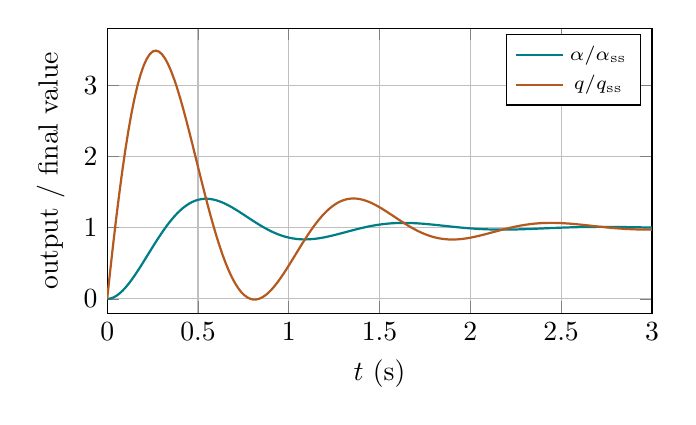
\begin{tikzpicture}
\begin{axis}[width=8.5cm,height=5.2cm,xlabel={$t\ (\mathrm{s})$},ylabel={output / final value},xmin=0,xmax=3,ymin=-.2,ymax=3.8,grid=major,legend style={font=\scriptsize}]
\addplot[teal,thick,domain=0:3,samples=180]{1-exp(-1.65536*x)*(cos(deg(5.7703*x))+1.65536/5.7703*sin(deg(5.7703*x)))};
\addlegendentry{$\alpha/\alpha_{\rm ss}$}
\addplot[orange,thick,domain=0:3,samples=180]{1+exp(-1.65536*x)*(-cos(deg(5.7703*x))+(36.047*.67-1.65536)/5.7703*sin(deg(5.7703*x)))};
\addlegendentry{$q/q_{\rm ss}$}
\end{axis}
\end{tikzpicture}
\end{column}
\begin{column}{.37\textwidth}
\small
零初值、小尾翼階躍，兩個輸出各自除以穩態值。
\bi\item 迎角峰值約 1.406。
\item 俯仰率峰值約 3.485，約出現在 0.267 秒。
\item 差別來自輸出零點，不是極點改變。
\item 這是簡化模型的響應，不代表真機實測。\ei
\end{column}
\end{columns}
}

\section{3.6 橫向控制}
\bookslide{坡度轉彎的力平衡}{3.6.1，pp. 148--149}{
考慮協調、等速、等高度轉彎。用 $L_{\rm lift}$ 表示總升力，避免與滾轉力矩 $L$ 混淆。
\[L_{\rm lift}\cos\phi=mg,\qquad
L_{\rm lift}\sin\phi=mV_T\dot\psi.\]
\[\boxed{\dot\psi=\frac{g\tan\phi}{V_T}},\qquad
\boxed{R=\frac{V_T^2}{g\tan\phi}},\qquad
\boxed{n=\frac{L_{\rm lift}}{mg}=\sec\phi}.\]
\bi
\item 升力的水平分量提供向心力，垂直分量仍須支撐重量。
\item 固定坡度時，速度越快，轉彎率越小、半徑越大。
\item 不能只增加坡度而不增加升力，否則會損失高度。
\ei
}
\originalfigure{3.33}{協調水平轉彎的受力}{149}{fig-3-33.png}{水平升力提供向心力，垂直分量平衡重量。}{}

\bookslide{轉彎算例與數值核對}{3.6.1，p. 149；補充計算}{
\small
$\phi=60^\circ$、$V_T=100\ \mathrm{m/s}$、$g=9.81\ \mathrm{m/s^2}$：
\[\begin{aligned}
n&=\sec60^\circ=2,\\
a_{\rm centripetal}&=g\tan60^\circ=1.732g,\\
\dot\psi&=\frac{9.81\tan60^\circ}{100}
=0.1699\ \mathrm{rad/s}=9.74^\circ/\mathrm{s},\\
R&\simeq588.5\ \mathrm{m}.
\end{aligned}\]
\key{核對提醒}教材列出的轉彎率為 $10.4^\circ/\mathrm{s}$。依同頁公式與 $100\ \mathrm{m/s}$ 重算得到約 $9.74^\circ/\mathrm{s}$。即使用 $g\simeq10$，也約為 $9.92^\circ/\mathrm{s}$。
}
\bookslide{協調轉彎需要哪些輸入？}{3.6.1，pp. 149--150}{
\bi
\item 副翼先建立滾轉角速度，到達所需坡度後將桿移回配平附近，以停止繼續滾轉。
\item 升降舵增加迎角與升力，以維持高度並產生所需向心力。
\item 方向舵修正副翼引起的偏航與側滑，使轉彎接近協調。
\item 油門增加推力以補償阻力增加，維持真空速。
\ei
\key{飛行員感受到的力}協調轉彎時，重力與慣性效果的合成感受大致沿機體法向，理想上沒有明顯側向滑動感。高 $g$ 轉彎仍需足夠升力與推力。
}
\bookslide{純滾轉的一階近似}{3.6.1，p. 150，式 (3.67)--(3.69)}{
忽略側滑與偏航耦合：
\[I_x\dot p=L_\xi\xi+L_pp,\qquad L_p<0.\]
\[\frac{p(s)}{\xi(s)}=\frac{L_\xi}{I_xs-L_p}
=\frac{K_R}{1+T_Rs},\quad
T_R=-\frac{I_x}{L_p}>0,\quad K_R=-\frac{L_\xi}{L_p}.\]
對階躍 $\xi_0$、零初值：
\[p(t)=K_R\xi_0(1-e^{-t/T_R}).\]
\key{核對提醒}保留導數正負號時，穩態增益必須為 $-L_\xi/L_p$。教材式 (3.68)--(3.69) 的正負號需要配合其大小值約定閱讀。
}
\originalfigure{3.34}{副翼階躍與滾轉率}{151}{fig-3-34.png}{將原圖的時間常數與漸近穩態值，對照一階響應公式。}{}

\bookslide{滾轉率與坡度是不同的輸出}{3.6.1，pp. 150--151；補充積分}{
\begin{columns}[T]
\begin{column}{.55\textwidth}
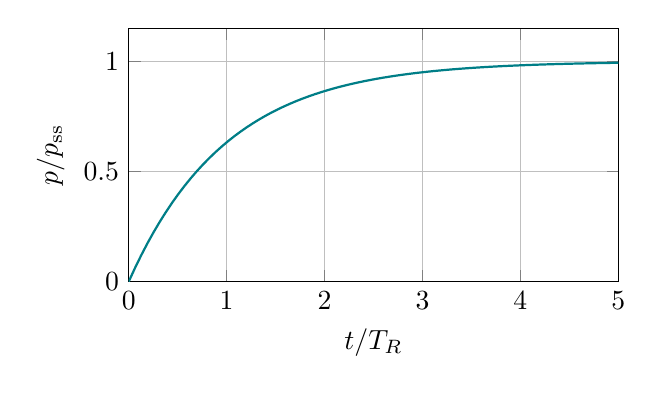
\begin{tikzpicture}
\begin{axis}[width=7.8cm,height=4.8cm,xlabel={$t/T_R$},ylabel={$p/p_{\rm ss}$},xmin=0,xmax=5,ymin=0,ymax=1.15,grid=major]
\addplot[teal,thick,domain=0:5,samples=80]{1-exp(-x)};
\end{axis}
\end{tikzpicture}
\end{column}
\begin{column}{.41\textwidth}
\small
\bi\item 一個時間常數後達穩態值的約 $63.2\%$。
\item 約 $3T_R$ 達 $95\%$。
\item 坡度為 $\phi(t)=\phi(0)+\int_0^t p(\tau)\,\dd\tau$。
\item 固定非零副翼在此模型中會持續滾轉，不會自動停在固定坡度。\ei
\end{column}
\end{columns}
}
\bookslide{方向舵的主要任務}{3.6.2，pp. 150--151}{
\bi
\item 修正副翼造成的偏航力矩，協助完成協調轉彎。
\item 抑制不希望出現的側滑，也能在需要時主動建立側滑。
\item 抵銷多發飛機單邊推力損失或非對稱外掛造成的偏航力矩。
\item 在側風落地的教材情境中，調整航向與跑道方向的對準關係。
\ei
\key{為何通常不用方向舵平轉？}機身與垂尾能提供的側向力遠小於主翼可提供的升力，且平轉會造成明顯側向加速度，效率與舒適性都較差。
}
\bookslide{純偏航模型的角度符號}{3.6.3，p. 152；核對角度約定}{
\small
以一般 $\beta=v/U$ 為側滑角，若速度向量的方向固定，而機頭向右偏航 $\psi>0$，則小角度下
\[\beta\simeq-\psi,\qquad v\simeq-U\psi.\]
所以在 $N_v>0$ 表示方向穩定的慣例下：
\[I_z\ddot\psi=N_v(-U\psi)+N_r\dot\psi,\qquad N_r<0,\]
\[\boxed{\ddot\psi+\frac{-N_r}{I_z}\dot\psi+\frac{N_vU}{I_z}\psi=0}.\]
\key{教材對照}教材寫 $\beta=\psi$ 並用 $N_v<0$ 表示恢復作用，這等效於另一個角度／導數正方向。不能把它與前面的 $v$ 慣例直接混用。
}
\bookslide{偏航振盪的自然頻率與阻尼}{3.6.3，pp. 152--153；一致符號推導}{
從前頁帶符號方程可得
\[\omega_{n,y}=\sqrt{\frac{N_vU}{I_z}},\qquad
\zeta_{d,y}=\frac{-N_r}{2\sqrt{I_zN_vU}}.\]
\bi
\item 垂尾恢復作用提供「剛度」，偏航慣性提供振盪的慣性，$N_r$ 提供阻尼。
\item 教材列舉純偏航振盪週期約 3--10 秒，阻尼不足時需要 yaw damper。
\item 教材的負 $N_v$ 慣例應改寫為 $\omega_n=\sqrt{-N_vU/I_z}$。同頁平方根式遺漏的符號不能照抄。
\item 若比較不同速度，必須同時更新 $N_v,N_r$。固定導數下的速度比例不能直接當作全包線規律。
\ei
}
\bookslide{Dutch roll、滾轉衰減與螺旋模態}{3.6.4，p. 153}{
\small
\begin{tabular}{p{.20\textwidth}p{.65\textwidth}}
\toprule 模態 & 物理描述\\\midrule
Dutch roll & 側滑、偏航與滾轉耦合的振盪。後掠與上反角效應影響各運動分量的比例。\\
Roll subsidence & 主要表現為滾轉率擾動快速衰減，常可用一階近似。\\
Spiral mode & 慢速的坡度、偏航與側滑演變，可能緩慢發散，教材例子時間尺度約半分鐘到一分鐘。\\\bottomrule
\end{tabular}
\key{相位提醒}教材用滾轉與偏航約相差 $90^\circ$ 作直觀描述。實際幅比與相位取決於模態特徵向量與觀測變數，不是所有飛機都精確相同。
}
\bookslide{橫向模型階數的核對}{3.4.5 與 3.6.4，pp. 133、153}{
\bi
\item p. 133 的 $\mathbf x=[v,p,r,\phi]^T$ 是四個狀態，因此 $\det(sI-A)$ 最高為四次。
\item 一般可用一對 Dutch roll 根，加上一個 roll 根與一個 spiral 根理解這個四階模型。
\item 若額外加入不回饋其他狀態的航向 $\dot\psi=r$，五階擴充模型會多一個零特徵值。
\item p. 153 列出五階分解，含另一個有限的 yaw subsidence 因子，與先前四階矩陣不能直接一一對上。
\ei
\key{使用原則}依實際採用的狀態方程計算極點。若要使用另一個五階模型，需先交代新增狀態與動態，不能只把五個模態硬套上四階矩陣。
}

\section{3.7 動力操縱與 PCU}
\bookslide{Power Control Unit 的作用}{3.7.1，pp. 154--155}{
\bi
\item 高速飛行時操縱面載荷很大，飛行員通常無法直接用人力驅動。
\item PCU 利用液壓能量產生大致動力，飛行員透過連桿移動小型伺服閥來發出命令。
\item 活塞移動透過機械回授逐漸關閉閥口，使活塞位置追隨輸入位置。
\item 教材的全動力系統要求避免操縱面反向驅動操縱機構，以處理回傳與顫振問題。
\ei
\key{能量與訊號}桿位移提供位置命令，液壓供應提供作動能量。機械傳令與液壓放大可以同時存在，並不等同於 FBW。
}
\originalfigure{3.35}{機械傳令的動力操縱系統}{154}{fig-3-35.png}{從飛行員操縱器沿連桿追到各操縱面的 PCU。}{Courtesy of BAE Systems.}

\bookslide{PCU 的力量與獨立供應}{3.7.1，p. 155}{
\bi
\item 教材典型液壓壓力約 $200\ \mathrm{bar}=20\ \mathrm{MPa}$。活塞面積決定可用力的尺度。
\item 兩套串聯致動結構與獨立液壓供應，用來提高失效後的控制能力。
\item 閥芯正常操縱力很小，但連桿仍可能需承受較大的人工作用力，以處理教材所述的卡閥情境。
\ei
\[F\simeq\Delta P\,A.\]
\key{補充算例}$\Delta P=20\ \mathrm{MPa}$、$A=10\ \mathrm{cm^2}=10^{-3}\ \mathrm{m^2}$ 時，$F\simeq20\ \mathrm{kN}$。這是面積與壓差的尺度估算，實際載荷須扣除回油壓與損失。
}
\bookslide{PCU 位置回授的幾何關係}{3.7.2，pp. 155--156，式 (3.72)}{
教材連桿幾何使閥口位移為
\[x_\varepsilon=\frac{x_i-Gx_o}{G+1}.\]
\bi
\item $x_i$：輸入桿位移。$x_o$：輸出活塞位移。$G$：教材定義的連桿比例。
\item 若輸入與回授尚未平衡，$x_\varepsilon\ne0$，液壓流動使活塞移動。
\item 理想穩態下，閥口重新關閉：$x_i-Gx_o=0$，所以 $x_o=x_i/G$。
\item 這是位置負回授，幾何比例決定 DC 增益，而液壓流量能力決定反應速度。
\ei
}
\originalfigure{3.36}{PCU 閥口與活塞回授}{155}{fig-3-36.png}{先辨認輸入、閥芯、液壓腔及活塞，再核對機械回授路徑。}{}

\bookslide{液壓流量如何形成一階模型}{3.7.2，pp. 156--157}{
\small
教材假設：方形且對稱的閥口、油液不可壓縮、外部負載與慣性可忽略、回油壓近似零。
\[a_{\rm port}=K_1x_\varepsilon,\qquad
v_{\rm oil}=K_2\sqrt{\Delta P}.\]
進出流量相等且活塞受力平衡時，
\[P_1=P_2=P_s/2,\qquad
Q_h=A\dot x_o=K_1K_2x_\varepsilon\sqrt{P_s/2}.\]
\[\dot x_o=K_vx_\varepsilon,\qquad K_v=\frac{K_1K_2}{A}\sqrt{\frac{P_s}{2}}.\]
\key{符號提醒}$Q_h$ 是液壓體積流率，與本章氣動壓力 $Q$ 不同。
}
\bookslide{PCU 傳遞函數、頻寬與相位}{3.7.2，p. 157，式 (3.73)--(3.75)}{
\[\dot x_o=\frac{K_v}{G+1}(x_i-Gx_o)\]
\[\boxed{\frac{x_o}{x_i}=\frac{1/G}{1+T_{\rm act}s}},
\qquad T_{\rm act}=\frac{G+1}{GK_v}.\]
\bi
\item 教材例子 $T_{\rm act}=0.1\ \mathrm{s}$，$-3\ \mathrm{dB}$ 頻率 $\omega_b=10\ \mathrm{rad/s}$，約 $1.59\ \mathrm{Hz}$。
\item $1\ \mathrm{Hz}$ 的相位為 $-\tan^{-1}(2\pi\cdot1\cdot0.1)\simeq-32.1^\circ$。
\item 致動器不是瞬間完成指令。相位延遲會降低外部飛控回路可用的穩定裕度。
\item 有負載、油液彈性、速率限制或間隙時，一階模型可能不足。
\ei
}

\section{3.8 穩定增強系統}
\bookslide{SAS 以回授建立額外阻尼}{3.8.1，pp. 157--158}{
\bi
\item 角速度感測器量測 $p,q,r$，控制器產生相對應的操縱面修正。
\item 修正輸入透過差動機構與飛行員命令相加，產生反抗角速度的附加力矩。
\item Pitch damper、roll damper、yaw damper 分別補充相應軸的阻尼。
\item Yaw damper 特別用於抑制 Dutch roll；強滾轉偏航耦合時，可能還需 roll damper。
\ei
\key{局部等效}若 $\eta=\delta_i-G_q q$ 且 $M_\eta>0$，則有效俯仰阻尼導數為 $M_{q,\rm eff}=M_q-M_\eta G_q$，變得更負。
}
\originalfigure{3.37}{簡單穩定增強系統}{158}{fig-3-37.png}{比較飛行員輸入和角速度回授如何在差動機構中合成。}{}

\bookslide{有限權限的意義}{3.8.1，p. 158}{
\bi
\item 有限權限 SAS 適合原本仍可飛、但部分包線阻尼不足的飛機。
\item 限制 SAS 的最大舵面修正量，可限制失效時造成的運動，使飛行員能解除並接手。
\item 教材給出的典型權限，相當於約 $\pm0.5g$ 的操縱面作用，但不同系統並非都採同一數值。
\item 單通道系統沒有平行備援，故失效安全依賴有限權限、可解除性與基本飛機的可控性。
\ei
\key{不能混淆}有限權限是「可施加多少控制」，單通道是「有幾條獨立鏈路」。兩者描述不同設計面向。
}
\bookslide{Wash-out 為何讓偏航阻尼器不抵抗轉彎？}{3.8.1，pp. 159--160}{
持續轉彎有非零的平均偏航率。若直接用純比例負回授，SAS 會試圖抵抗這個飛行員有意要求的轉彎。
\[
H_w(s)=\frac{T_ws}{1+T_ws}
\quad\text{（補充：典型洗出濾波器形式）}
\]
\bi
\item $H_w(0)=0$：穩態 DC 成分被去除。
\item 在目標振盪頻帶保留足夠角速度訊號，讓阻尼器針對振盪動作。
\item 再加高頻低通，例如 $1/(1+T_fs)$，形成低頻與高頻都衰減的頻率選擇。
\item 通帶仍可能有幅值與相位誤差，設計時要計算實際濾波器，不能假設一定零相移。
\ei
}
\originalfigure{3.38}{洗出與高頻截止的頻率特性}{159}{fig-3-38.png}{低頻抑制持續轉彎成分，高頻截止降低雜訊與結構模態的影響。}{}

\bookslide{結構模態、濾波與增益排程}{3.8.1，pp. 158--160}{
\bi
\item 致動器施力會使有限剛度的機體彎曲，陀螺儀可能量到彈性振動而不只是剛體轉動。
\item 若回授在結構頻率仍有足夠增益與不利相位，控制器可能激發該結構模態。
\item 低通抑制高頻訊號；notch filter 在特定結構共振附近提供較深的衰減。
\item 高度、速度改變會改變操縱效率，教材以切換兩三組增益說明簡單的增益排程。
\ei
\key{取捨}濾波抑制雜訊與共振，也會增加相位延遲。不能只以「濾得越多越好」決定控制器。
}
\bookslide{俯仰 SAS 的閉迴路推導}{3.8.1.1，pp. 160--161}{
\small
基本飛機模型與增穩律：
\[G_p(s)=\frac{K(1+T_2s)}{s^2+A_1s+A_2},\qquad
\eta=\delta_i-G_qq.\]
代入 $q=G_p(\delta_i-G_qq)$ 並整理：
\[\boxed{\frac q{\delta_i}=
\frac{K(1+T_2s)}
{s^2+(A_1+KT_2G_q)s+(A_2+KG_q)}}.\]
\[\omega_{n,\rm cl}^2=A_2+KG_q,\quad
2\zeta_{d,\rm cl}\omega_{n,\rm cl}=A_1+KT_2G_q.\]
\key{看係數的意義}速率回授同時改變阻尼係數與自然頻率，也改變 DC 增益 $K/(A_2+KG_q)$。這個推導仍忽略致動器、濾波器及感測器延遲。
}
\originalfigure{3.39}{俯仰率增穩回路}{161}{fig-3-39.png}{追蹤飛行員指令、俯仰率量測與增穩舵角的負回授。}{}

\bookslide{SAS 算例：教材的設計鏈}{3.8.1.1，p. 161}{
教材採用 $K=87$、$T_2=0.67$、$\omega_n=6$、$\zeta_d=0.2$，要求 $\zeta_{d,\rm cl}=0.7$：
\[
1.4\sqrt{36+87G_q}=2.4+87(0.67)G_q.
\]
\bi
\item 解得 $G_q$ 約 $0.12\ \mathrm{s}$，亦可寫成「度尾翼／（度每秒俯仰率）」。
\item 教材四捨五入後列出 $\omega_{n,\rm cl}\simeq6.8\ \mathrm{rad/s}$。
\item 閉迴路分母約為 $s^2+9.5s+46$。
\item 此設計沿用前面偏低的阻尼估計，故要與重算模型分開閱讀。
\ei
}
\bookslide{SAS 算例：依重算模型重新設計}{3.8.1.1；補充一致重算}{
\small
使用 $A_1=3.3107$、$A_2=36.0470$、$K=87.0647$，仍要求 $\zeta_{d,\rm cl}=0.7$：
\[
1.4\sqrt{36.0470+87.0647G_q}
=3.3107+87.0647(0.67)G_q.
\]
取符合原式且為正的解：
\[
\boxed{G_q=0.1045\ \mathrm{s}},\quad
\boxed{\omega_{n,\rm cl}=6.7190\ \mathrm{rad/s}}.
\]
\[
\frac q{\delta_i}\simeq
\frac{87.0647(1+0.67s)}
{s^2+9.4067s+45.1454}.
\]
\key{結果差異}重算的基本飛機原本阻尼較高，因此達到同樣目標需要的增穩增益較小。這個數值僅供理解本章簡化設計流程。
}
\bookslide{極點改善不等於所有輸出都同樣改善}{3.8.1.1，pp. 160--162；補充比較}{
\small
\begin{tabular}{lcc}
\toprule 量 & 重算的基本飛機 & 加入 $G_q=0.1045$\\\midrule
$\omega_n\ (\mathrm{rad/s})$ & 6.004 & 6.719\\
$\zeta_d$ & 0.276 & 0.700\\
$q$ 的 DC 增益 $(\mathrm{s^{-1}})$ & 2.415 & 1.929\\
約略包絡時間常數 $1/(\zeta_d\omega_n)$ & 0.604 s & 0.213 s\\\bottomrule
\end{tabular}
\bi
\item 衰減變快，但相同輸入的穩態俯仰率也降低了。
\item $q$ 通道的零點仍存在，不能把「阻尼比 0.7」直接翻譯為 $q$ 的固定過衝百分比。
\item 若致動器有顯著延遲，必須把其狀態納入閉迴路，再檢查穩定性。
\ei
}
\originalfigure{3.40}{加入增穩前後的響應}{162}{fig-3-40.png}{此圖為教材示意，用來比較振盪衰減，不當作本筆記重算模型的數值曲線。}{}

\bookslide{全權限 SAS 與三重冗餘}{3.8.2，p. 162}{
\bi
\item 某些飛行狀態需要大幅甚至全權限的穩定修正，單靠限制舵角不足以保證失效後安全。
\item 教材的 triplex 概念包含三條獨立感測、計算與致動通道，以及獨立供電／液壓。
\item 交叉比較可辨識單一離群通道，隔離後剩下雙通道。
\item 教材描述的後續處置是離開強依賴增穩的飛行區域，降低在剩餘冗餘下運作的風險。
\ei
\key{架構限制}三條通道不會自動消除共同原因失效。教材描述的第二次失效「被動停止」也依賴實際致動與監控架構，不能只由通道數推論。
}
\bookslide{固定翼單元的整合檢查}{3.2--3.8，pp. 101--162}{
\begin{enumerate}\setlength{\itemsep}{7pt}
\item 為何不能只把 $\lvert M_q\rvert$ 無限加大？\\
\textbf{致動器與濾波延遲、結構模態、控制權限和操縱增益都會限制可用回授。}
\item 為何 yaw damper 需要 wash-out？\\
\textbf{區分希望抑制的振盪，與飛行員持續要求的轉彎。}
\item 為何 full authority 要提高失效存活能力？\\
\textbf{錯誤指令可能用全舵量影響飛機，且某些狀態無法靠人力及時接手。}
\item 前面建立氣動導數有什麼用途？\\
\textbf{把控制面、感測回授與飛機的實際動態連成可分析的模型。}
\end{enumerate}
}

\section{講義核對}
\slide{角速度與 Euler 角變化率}{Handout 4，PDF pp. 13--18；概念整理與補充推導}{
\small
\bi
\item $p,q,r$ 是機體軸角速度分量，$\dot\phi,\dot\theta,\dot\psi$ 是姿態參數的時間導數。
\item 兩者透過姿態相關的矩陣轉換，通常不相等。
\item 小角近似應作用在擾動量，而配平俯仰角本身不一定很小。
\ei
\key{閱讀重點}使用 Euler 轉換時，先確認旋轉順序、方向與姿態的定義。
}
\handoutfigure{16}{角速度與 Euler 角變化率}{handout04-p016.png}
\handoutfigure{17}{角速度與 Euler 角變化率}{handout04-p017.png}
\slide{自我檢查：角速度與 Euler 角變化率}{依 Handout 範圍自編問題與參考解答}{
\small
\key{先自行作答}
標準 3--2--1 Euler 定義下，當 $\phi=0$ 但 $\theta\ne0$，是否可直接令 $r=\dot\psi$？
\key{參考解答}
不可以。此時 $r=\dot\psi\cos\theta$，而 $p=\dot\phi-\dot\psi\sin\theta$。只有額外的小姿態近似才可把部分關係簡化。
}
\slide{剛體假設與慣性乘積}{Handout 4，PDF pp. 19--30；概念整理與補充推導}{
\small
\bi
\item 短期飛行動力學常假設質量與慣性固定、機體近似剛體，再用 Newton--Euler 方程分析。
\item 對 xz 平面左右對稱，$I_{xy}$ 與 $I_{yz}$ 消失，$I_{xz}$ 仍可能非零。
\item 對稱性不表示質量必須均勻分布，取主慣性軸才可進一步使全部慣性乘積為零。
\ei
\key{閱讀重點}簡化之前要明確說明採用機體幾何軸還是主慣性軸。
}
\handoutfigure{27}{剛體假設與慣性乘積}{handout04-p027.png}
\handoutfigure{29}{剛體假設與慣性乘積}{handout04-p029.png}
\slide{自我檢查：剛體假設與慣性乘積}{依 Handout 範圍自編問題與參考解答}{
\small
\key{先自行作答}
為什麼 $qW$ 線性化時不能整項刪掉？若 $Q_e=0$，$W=W_e+w$，展開 $QW$。
\key{參考解答}
$QW=(Q_e+q)(W_e+w)=qW_e+qw$。$qW_e$ 是一階量，應保留。$qw$ 是兩個擾動相乘的二階量，才在一階線性化中忽略。
}
\slide{控制面也會產生力}{Handout 4，PDF pp. 31--46；概念整理與補充推導}{
\small
\bi
\item 氣動穩定導數表示狀態改變對力及力矩的局部影響，控制導數表示操縱輸入的影響。
\item 講義 p. 44「控制面只能施加力矩」應視為某些模型的簡化，升降舵等同時會產生氣動力。
\item 原筆記保留直接尾翼力與忽略直接力的兩種推導，便於看出簡化改變什麼。
\ei
\key{閱讀重點}衍生模型要同時檢查省略項、導數定義及其單位。
}
\handoutfigure{44}{控制面也會產生力}{handout04-p044.png}
\slide{自我檢查：控制面也會產生力}{依 Handout 範圍自編問題與參考解答}{
\small
\key{先自行作答}
若 $Z_{\delta_e}\ne0$，升降舵階躍對瞬時垂直加速度與後續俯仰可能有什麼不同影響？
\key{參考解答}
舵面直接氣動力可立即改變法向加速度，同時俯仰力矩改變角速度與迎角，後續主翼升力再改變。只保留力矩的模型會省略前者。
}
\slide{狀態空間中的輸出與可量測性}{Handout 4，PDF pp. 47--59；概念整理與補充推導}{
\small
\bi
\item 狀態式為 $\dot{\mathbf x}=A\mathbf x+B\mathbf u$，輸出式為 $\mathbf y=C\mathbf x+D\mathbf u$。
\item 只有把全部狀態直接定義為輸出時才有 $C=I,D=0$，實際感測器未必直接量到全部狀態。
\item 縱向與橫向解耦依賴對稱性、配平狀態及小擾動等假設，大側滑或強耦合時需重檢查。
\ei
\key{閱讀重點}模型狀態、感測器量測及顯示輸出需要分別定義。
}
\handoutfigure{51}{狀態空間中的輸出與可量測性}{handout04-p051.png}
\handoutfigure{59}{狀態空間中的輸出與可量測性}{handout04-p059.png}
\slide{自我檢查：狀態空間中的輸出與可量測性}{依 Handout 範圍自編問題與參考解答}{
\small
\key{先自行作答}
自編例：$\mathbf x=[u,w,q,\theta]^T$，只量到 $q$ 與 $\theta$，寫出 $C$。
\key{參考解答}
$C=\begin{bmatrix}0&0&1&0\\0&0&0&1\end{bmatrix}$。若假設量測無直接輸入通道，$D$ 為相應尺寸零矩陣。這不表示其他狀態不存在。
}
\section{算例與響應}
\slide{二階分母與傳遞函數}{Handout 4，PDF pp. 60--66；概念整理與補充推導}{
\small
\bi
\item 講義算例的短週期分母為 $s^2+0.8898s+4.895$。
\item 對照 $s^2+2\zeta\omega_ns+\omega_n^2$，可得到自然頻率及阻尼比。
\item 分子零點會影響階躍響應，不能只從分母阻尼比直接套標準無零點過衝公式。
\ei
\key{閱讀重點}極點決定模態，輸入與輸出的選擇及零點決定該模態如何呈現。
}
\handoutfigure{60}{二階分母與傳遞函數}{handout04-p060.png}
\handoutfigure{65}{二階分母與傳遞函數}{handout04-p065.png}
\slide{自我檢查：二階分母與傳遞函數}{依 Handout 範圍自編問題與參考解答}{
\small
\key{先自行作答}
依上述分母求 $\omega_n$、$\zeta$ 與極點，並說明穩定性。
\key{參考解答}
$\omega_n=\sqrt{4.895}=2.2125\,\mathrm{rad/s}$，$\zeta=0.8898/(2\omega_n)=0.2011$。極點約 $-0.4449\pm j2.1673$，均在左半平面，屬穩定的欠阻尼模態。
}
\section{講義核對}
\slide{SAS 的阻尼方向}{Handout 4，PDF pp. 67--68；概念整理與補充推導}{
\small
\bi
\item SAS 以運動感測回授產生操縱修正，改善選定模態的阻尼及穩定性。
\item 講義 p. 68 的「Reduce the damping ratio」不宜作為一般目標，對欠阻尼模態通常希望增加有效阻尼。
\item 回授符號必須連同舵角正方向與控制導數檢查，不能只看到負號就保證是穩定回授。
\ei
\key{閱讀重點}增穩仍要考慮致動器、延遲、結構模態及行程限制。
}
\handoutfigure{67}{SAS 的阻尼方向}{handout04-p067.png}
\handoutfigure{68}{SAS 的阻尼方向}{handout04-p068.png}
\slide{自我檢查：SAS 的阻尼方向}{依 Handout 範圍自編問題與參考解答}{
\small
\key{先自行作答}
自編模型 $\dot q=-0.5q+2\delta_e$，取 $\delta_e=-kq$。求閉迴路極點。
\key{參考解答}
$\dot q=-(0.5+2k)q$，極點為 $-(0.5+2k)$。在此符號與無延遲模型中 $k>0$ 增快衰減。實際系統不能據此無限制加大增益。
}
\section{複習與來源}
\slide{整合複述檢查}{Handout 4 全份複習}{
\bi
\item 選一項系統功能，說明輸入、輸出、座標、單位與資料來源。
\item 找出一個公式，逐一解釋每個符號，再說明它使用哪些假設。
\item 選一個故障或誤差，追蹤它如何影響下游功能，以及可以用什麼獨立資訊核對。
\item 重做本份的自我檢查，再對照講義與相關公式。
\ei
}
\slide{來源與後續閱讀}{Handout 4 與隨附教材}{
\small
\bi
\item 主要來源：賴盈誌老師，CA7528 Digital Avionics，Handout 4。原始檔保留於上一層資料夾。
\item 版型與重用內容：既有 Chapter03\_SelfStudy\_LaTeX。Handout 3、4 沿用相關章節及其原圖。
\item 第三章重用內容來源：R. P. G. Collinson，\textit{Introduction to Avionics Systems}，第 3 版。
\item 本筆記的重算、核對與延伸為自讀整理，並非授課教師或出版社正式勘誤。
\item 原圖內來源標示與圖說保留，新增題目與參考解答已另行標明。
\ei
}
\end{document}
